\documentclass{article}
\usepackage[utf8]{inputenc}
\usepackage{amsmath}
\usepackage{amsfonts}
\usepackage[margin=0.7in]{geometry}
\usepackage{graphicx}
\usepackage{amssymb}
\usepackage{gensymb}
\usepackage{booktabs}
\usepackage{wrapfig}
\usepackage{caption}
\usepackage[export]{adjustbox}
\usepackage[pdfborder={0 0 0}]{hyperref}
\usepackage{pdfpages}
\usepackage{fancyhdr}
\usepackage{parskip}
\usepackage{lastpage}
\usepackage{listings}
\usepackage{multirow}
\usepackage{xifthen}
\usepackage{xcolor}
\usepackage{mathtools}
\graphicspath{{images/}}
\pagestyle{fancy}

\begin{document}
\title{ØkIntro Aflevering 3}
\author{Carl-Emil Rohde - kvb125}
\date{December 2022}
\maketitle

\section*{Opgave 1}
\subsection*{1.1}
Jeg opstiller et minimeringsproblem, hvor jeg minimerer virksomhedens omkostninger, $O=w_1x_1+w_2x_2$ ved produktion:
\begin{equation}
    min(x_x,x_2) w_1x_1+w_2x_2
\end{equation}
Jeg løser dette ved brug af Lagrange, under bibetingelse af produktionsfunktionen $x_1^\alpha x_2^{1-\alpha}$: 
\begin{equation}
    L = x_1w_1+x_2w_2 - \lambda (x_1^\alpha x_2^{1-\alpha}- y)
\end{equation}
Partiel differentiering for alle variable:
\begin{equation}
    1) \frac{\partial L}{\partial x_1} = w_1-\lambda \alpha x_2^{1-\alpha} x_1^{\alpha-1}=0 \\
\end{equation}
\begin{equation}
    2) \frac{\partial L}{\partial x_2}=w_2-\lambda(1-\alpha) x_1^\alpha x_2^{-\alpha}=0 \\
\end{equation}
\begin{equation}
    3) \frac{\partial L}{\partial \lambda}=y-x_1^\alpha x_2^{1-\alpha}=0 \Leftrightarrow y=x_1^\alpha x_2^{1-\alpha}
\end{equation}

For ligning 1) og 2), isolerer jeg nu $w_1$ og $w_2$:
\begin{equation}
    w_1=\lambda \alpha x_1^{\alpha-1} x_2^{1-\alpha}
\end{equation}
\begin{equation}
    w_2=\lambda x_1^{\alpha-1}(1-\alpha) x_2^{-\alpha}
\end{equation}
Nu dividerer jeg $w_1$ med $w_2$:
\begin{equation}
    \frac{w_1}{w_2}=\frac{\lambda \alpha x_1^{\alpha-1} x_2^{1-\alpha}}{\lambda x_1^{\alpha-1}(1-\alpha) x_2^{-\alpha}} \Leftrightarrow
\end{equation}
\begin{equation}
    \frac{\alpha x_1^{\alpha-1} x_2^{1-\alpha}}{x_1^{\alpha-1}(1-\alpha) x_2^{-\alpha}} \Leftrightarrow
\end{equation}
\begin{equation}
    \alpha \cdot \frac{1}{(1-\alpha)} \frac{x_1^{\alpha-1}}{x_1^\alpha} \frac{x_2^{1-\alpha}}{x_2^{-\alpha}} \Leftrightarrow
\end{equation}
\begin{equation}
    \frac{x_2}{x_1} \frac{\alpha}{(1-\alpha)}
\end{equation}
Jeg isolerer nu $x_1$ og $x_2$ i udtrykket $\frac{w_1}{w_2}=\frac{x_2}{x_1} \frac{\alpha}{(1-\alpha)}$
\\Først $x_1$:
\begin{equation}
    \frac{w_1}{w_2}=\frac{\alpha x_2}{x_1(1-\alpha)}
\end{equation}
bruger $\frac{a}{b}=\frac{c}{d} \Rightarrow a \cdot d=b \cdot c$
\begin{equation}
    w_1 x_1(1-\alpha)=w_2 \alpha x_2
\end{equation}
dividerer med $w_1(1-\alpha)$ på begge sider:
\begin{equation}
    \frac{w_1 x_1(1-\alpha)}{w_1(1-\alpha)}=\frac{w_2 \alpha x_2}{w_1(1-\alpha)}
\end{equation}
reducerer:
\begin{equation}
    x_1=\frac{w_2 \alpha x_2}{w_1(1-\alpha)}
\end{equation}

Nu for $x_2$:
\\Jeg starter fra (12), og starter med at gange med $x_1(-\alpha+1)$ på begge sider og reducerer:
\begin{equation}
    \alpha x_2=\frac{w_1 x_1(-\alpha+1)}{w_2}
\end{equation}
Dividerer med $\alpha$ på begge sider og reducerer:
\begin{equation}
    \frac{\alpha x_2}{\alpha}=\frac{\frac{w_1 x_1(-\alpha+1)}{w_2}}{\alpha} \Leftrightarrow x_2=\frac{x_1 w_1(-\alpha+1)}{\alpha w_2}
\end{equation}

Udtrykket for $x_2$ indsættes nu i produktionsfunktionen, og der isoleres for $x_1$:
\begin{equation}
    y=x_1^\alpha\left(\frac{w_1(1-\alpha)}{w_2 \alpha} x_1\right)^{1-\alpha} \Leftrightarrow
\end{equation}
\begin{equation}
    y=x_1^\alpha x_1^{1-\alpha}\left(\frac{w_1(1-\alpha)}{w_2 \alpha}\right)^{1-\alpha} \Leftrightarrow
\end{equation}
\begin{equation}
    \frac{y}{\left(\frac{w_1(1-\alpha)}{w_2 \alpha}\right)^{1-\alpha}}=x_1 \Leftrightarrow
\end{equation}
Udtrykket for $x_1$, bliver således:
\begin{equation}
    x_1(w_1, w_2, y) = y *\left(\frac{w_1(1-\alpha)}{w_2 \alpha}\right)^{-1+\alpha}
\end{equation}
Nu gør jeg det samme for $x_2$:
\begin{equation}
    y=\left(\frac{x_2 w_2 \alpha}{w_1(1-\alpha)}\right)^\alpha x_2^{1-\alpha}
\end{equation}
\begin{equation}
    y=\left(\frac{w_2 \alpha}{w_1(1-\alpha)}\right)^\alpha x_2^\alpha x_2^{1-\alpha}
\end{equation}
\begin{equation}
    \frac{y}{\left(\frac{w_2 \alpha}{w_1(1-\alpha)}\right)^\alpha}=x_2
\end{equation}
udtrykket for $x_2$, bliver således:
\begin{equation}
    x_2(w_1, w_2, y) = y *\left(\frac{w_2 \alpha}{w_1(1-\alpha)}\right)^{-\alpha}
\end{equation}

\subsection*{1.2}
For at finde elasticiteten, starter jeg med at finde et udtryk for $\frac{x_2}{x_1}$:
\begin{equation}
    \frac{x_2}{x_1} = \frac{y *\left(\frac{w_2 \alpha}{w_1(1-\alpha)}\right)^{-\alpha}}{y *\left(\frac{w_1(1-\alpha)}{w_2 \alpha}\right)^{-1+\alpha}} =\frac{w_1(1-\alpha)}{w_2 \alpha} \Rightarrow \frac{1-a}{(a)} \cdot\left(\frac{w_2}{w_1}\right)^{-1}
\end{equation}
(Jeg ved godt den sidste omskrivning herover, ikke gør udtrykket pænere, men fandt det nemmere at regne videre med.) 
\\Nu indsætter jeg dette udtryk, i udtrykket for elasticitet:
\begin{equation}
    \frac{\partial \frac{x_2}{x_1}}{\partial \frac{w_2}{w_1}} \frac{\frac{w_2}{w_1}}{\frac{x_2}{x_1}}=\frac{\partial \frac{1-a}{(a)} \cdot\left(\frac{w_2}{w_1}\right)^{-1}}{\partial \frac{w_2}{w_1}} \frac{\frac{w_2}{w_1}}{\frac{1-a}{(a)} \cdot\left(\frac{w_2}{w_1}\right)^{-1}}
\end{equation}
reducerer:
\begin{equation}
    \frac{\partial \frac{x_2}{x_1}}{\partial \frac{w_2}{w_1}} \frac{\frac{w_2}{w_1}}{\frac{x_2}{x_1}}=\frac{(1-a) \cdot\left(\frac{w_2}{w_1}\right)^{-2}}{a} \cdot \frac{\left(\frac{w_2}{w_1}\right)^2 \cdot a}{(1-a)} = -1
\end{equation}
Elasticiteten er altså bestemt til at være $-1$

\subsection*{1.3}
Jeg opskriver et udtryk, der beskriver den samlede andel input 1 udgør, af omkostningerne:
\begin{equation}
    \frac{w_1 x_1}{w_1 x_1+w_2 x_2}=\frac{1}{1+\frac{w_2 x_2}{w_1 x_1}}
\end{equation}
Nu indsætter jeg udtrykket for $\frac{x_2}{x_1}$:
\begin{equation}
    \frac{1}{1+\frac{w_2}{w_1} \cdot \frac{1-a}{(a)} \cdot\left(\frac{w_2}{w_1}\right)^{-1}} \Rightarrow
\end{equation}
Reducerer:
\begin{equation}
    \frac{1}{1+\frac{1-a}{(a)}}\Leftrightarrow\frac{1}{\frac{a+(1-a)}{(a)}}\Leftrightarrow\frac{a}{a+(1-a)}\Leftrightarrow\frac{a}{1}=a
\end{equation}
For den del af omkostningerne der bliver brugt på input 1, er elasticiteten altså $a$.

\subsection*{1.4}
Omkostningerne er normalt givet ved $c=w_1 x_1+w_2 x_2$. Jeg kender nu udtrykkende for hhv $x_1$ og $x_2$, og indsætter nu disse i udtrykket for omkostninger:
\begin{equation}
    c\left(w_1, w_2, y\right)=w_1 y *\left(\frac{w_1(1-\alpha)}{w_2 \alpha}\right)^{-1+\alpha}+w_2 y *\left(\frac{w_2 \alpha}{w_1(1-\alpha)}\right)^{-\alpha}
\end{equation}
\begin{equation}
    c\left(w_1, w_2, y\right)=y*(w_1 \left(\frac{w_1(1-\alpha)}{w_2 \alpha}\right)^{-1+\alpha}+w_2 \left(\frac{w_2 \alpha}{w_1(1-\alpha)}\right)^{-\alpha})
\end{equation}
Således bliver dette omkostningsfunktionen.

\subsection*{1.5}
For at vise, at virksomhedens marginalomkostninger er konstante i $y$, finder jeg den partielt afledte for omkostningsfunktionen med hensyn til $y$:
\begin{equation}
    \frac{\partial c}{\partial y}=w_1 \left(\frac{w_1(1-\alpha)}{w_2 \alpha}\right)^{-1+\alpha}+w_2 \left(\frac{w_2 \alpha}{w_1(1-\alpha)}\right)^{-\alpha}
\end{equation}
Ovenstående udtryk er uafhængigt af $y$. Dermed er det bevist, at marginalomkostningerne er konstante i $y$.



\section*{Opgave 2}
\subsection*{2.1}
Jeg antager at udbuddet er lig marginal omkostningerne. Jeg starter med at finde den partielt afledte for omkostningsfunktionen med hensyn til $y$:
\begin{equation}
    \frac{\partial C}{\partial y}=\frac{\frac{1+\alpha}{\alpha} * \alpha}{1+\alpha} y^{\frac{1+\alpha}{\alpha}-1} \Leftrightarrow 1 y^{\frac{1}{\alpha}+\frac{\alpha}{\alpha}-1} \Leftrightarrow y^{\frac{1}{\alpha}}
\end{equation}
Fordi $MC=p$ kan jeg opskrive:
\begin{equation}
    MC=y^\frac{1}{\alpha} \Leftrightarrow p=y^\frac{1}{\alpha} \Leftrightarrow y(p)=p^{\alpha}
\end{equation}
Således har jeg fundet den enkelte virksomheds udbudsfunktion:
$y(p)=p^{\alpha}$

\subsection*{2.2}
Jeg kan finde den enkelte virksomheds udbudselasticitet, med formlen: $\frac{\partial y}{\partial p} \frac{p}{y}$:
\begin{equation}
    \frac{\partial y}{\partial p} \frac{p}{y}=\frac{\partial y}{\partial p} \frac{p}{p^\alpha} = \frac{\alpha p^{\alpha-1} p^1}{p^\alpha} = \frac{\alpha p^\alpha}{p^\alpha} = \alpha p^{\alpha-\alpha} = \alpha
\end{equation}
Jeg ved fra opgavebeskrivelsen, at $\alpha>0$. Udbudselasticiteten går altså enten mod $0$ eller $\infty$, alt efter hvad $\alpha$ gør. Økonomisk kan dette fortolkes som virksomhedens villighed til at udbyde sine vare, alt afhængig af pris og omkostninger.

\subsection*{2.3}
Da alle virksomhederne har den samme udbudsfunktion, må industriens samlede udbud være givet ved udbudsfunktionen, ganget med antallet af virksomheder:
\begin{equation}
    Y(n, p)=n p^\alpha
\end{equation}
$n$ = antal virksomheder

\subsection*{2.4}
For at finde ligevægten i markedet, sætter jeg $udbud = efterspørgsel$:
\begin{equation}
    \frac{A}{p^\epsilon}=n p^\alpha
\end{equation}
Først finder jeg ligevægtsprisen ved at isolere $p$:
\begin{equation}
    \frac{A}{n}=p^\alpha p^\epsilon \Leftrightarrow \frac{A}{n}=p^{\alpha+\epsilon} \Leftrightarrow p^{LV}=\left(\frac{A}{n}\right)^{\frac{1}{\alpha+\epsilon}}
\end{equation}
Ligevægtsmængden finder jeg ved at indsætte $p^{LV}$ i udtrykket for industriens samlede udbud:
\begin{equation}
    Y^{LV}=n \cdot\left(\left(\frac{A}{n}\right)^{\frac{1}{a+\epsilon}}\right)^a \Leftrightarrow n \cdot\left(\frac{A}{n}\right)^{\frac{a}{a+\epsilon}}
\end{equation}

\subsection*{2.5}
Elasticiteten for ligevægtsprisen mht. $A$, er givet ved $\frac{\partial p^{LV}}{\partial A} \frac{A}{p^{LV}}$:
\begin{equation}
    \frac{\partial p^{LV}}{\partial A} \frac{A}{p^{LV}}=\frac{1}{a+\varepsilon} \frac{A^{\frac{1}{a+\varepsilon}-1}}{n^{\frac{1}{a+\varepsilon}}} \frac{A}{\left(\frac{A}{n}\right)^{\frac{1}{a+\varepsilon}}} \Leftrightarrow
\end{equation}
\begin{equation}
    \frac{A^{\frac{1}{a+\varepsilon}}}{\frac{(a+\varepsilon) n^{\frac{1}{a+\varepsilon}} A^{\frac{1}{a+\varepsilon}}}{n^{\frac{1}{a+\varepsilon}}}} \Leftrightarrow
\end{equation}
\begin{equation}
    \frac{1}{a+\varepsilon}
\end{equation}
Elasticiteten for ligevægtsprisen mht. A er dermed lig $ \frac{1}{a+\varepsilon}$

\subsection*{2.6}
I udtrykket for elasticiteten, kan jeg se, at for $a \rightarrow 0$, har vi at $\frac{1}{a+\epsilon} \rightarrow \frac{1}{\epsilon}$. For $a \rightarrow \infty$, har vi at $\frac{1}{a+\epsilon} \rightarrow 0$. Ved et højt elastisk udbud, det vil sige en høj $a$ værdi, vil efterspørgslen ikke have effekt på ligevægtsprisen, fordi den afhænger af $A$. Det modsatte er gældene for et inelastisk udbud, svarende til en lav $a$ værdi.

\subsection*{2.7}
Jeg antager først og fremmest, at ligevægtsprisen naturligvis er den samme for alle virksomheder på markedet, samt at profitten for alle virksomheder er ens. Profitten kan således udregnes, som værende forskellen mellem hhv. $pris * enheder \ produceret$ og omkostninger for den enkelte virksomhed. Det kan opskrives således: 
\begin{equation}
    \pi=p * y-C=p * p^a-\left(F+\frac{a}{1+a}\left(p^a\right)^{\frac{1+a}{a}}\right)
\end{equation}
Dette sætter jeg nu lig med $0$, og isolerer for $p$:
\begin{equation}
    p * p^a-\left(F+\frac{a}{1+a}\left(p^a\right)^{\frac{1+a}{a}}\right) = 0
\end{equation}
\begin{equation}
    p^{a+1}\left(1-\frac{a}{1+a}\right)=F
\end{equation}
\begin{equation}
p=\left(F\left(\frac{1+a}{1+a}-\frac{a}{1+a}\right)^{-1}\right)^{\frac{1}{a+1}}
\end{equation}
\begin{equation}
    p=\left(F\left(\frac{1}{1+a}\right)^{-1}\right)^{\frac{1}{a+1}}
\end{equation}
Ligevægtsprisen på lang sigt, bliver således:
\begin{equation}
    p^{LS}=(F(1+a))^{\frac{1}{a+1}}
\end{equation}

\subsection*{2.8}
For at bestemme elasticiteten for $p^{LS}$, skal jeg udregne $\frac{\partial p^{LS}}{\partial A} \frac{A}p^{LS}$. Jeg kan dog med det samme se, at $p^{LS}$ ikke er afhængig af $A$, hvorfor dette resultat må give $0$. 
\\
\\
Det vil altså sige, at prisen på lang sigt, er inelastisk. På lang sigt vil prisen på markedet altså ikke være påvirket af A eller ændringer i efterspørgslen. Hvis efterspørgslen stiger og A stiger med den, vil der blot komme en ny virksomhed ind på markedet, så prisen vil stadig nærme sig den langsigtede pris, som ikke afhænger af efterspørgslen eller A. Ligeledes, hvis efterspørgslen og A falder, vil nogle virksomheder forlade markedet, men prisen vil stadig nærme sig den langsigtede pris, som stadig ikke afhænger af efterspørgslen eller A.

\subsection*{2.9}
Jeg er i opgavebeskrivelsen givet efterspørgselsfunktionen for et produkt, så her isolerer jeg blot $p$:
\begin{equation}
    D(p)=\frac{A}{p^{\varepsilon}} \Leftrightarrow p=\left(\frac{A}{D(p)}\right)^{\frac{1}{\varepsilon}}
\end{equation}
For at finde udbudskurven (på kort sigt), isolerer jeg $p$ i udtrykket for industriens udbud:
\begin{equation}
    Y=n * p^a \Leftrightarrow p=\left(\frac{Y}{n}\right)^{\frac{1}{a}}
\end{equation}
Udbudskurven på lang sigt, må være $p^{LS}$
\\
\\
Jeg tegner det hele ind:

\begin{center}
    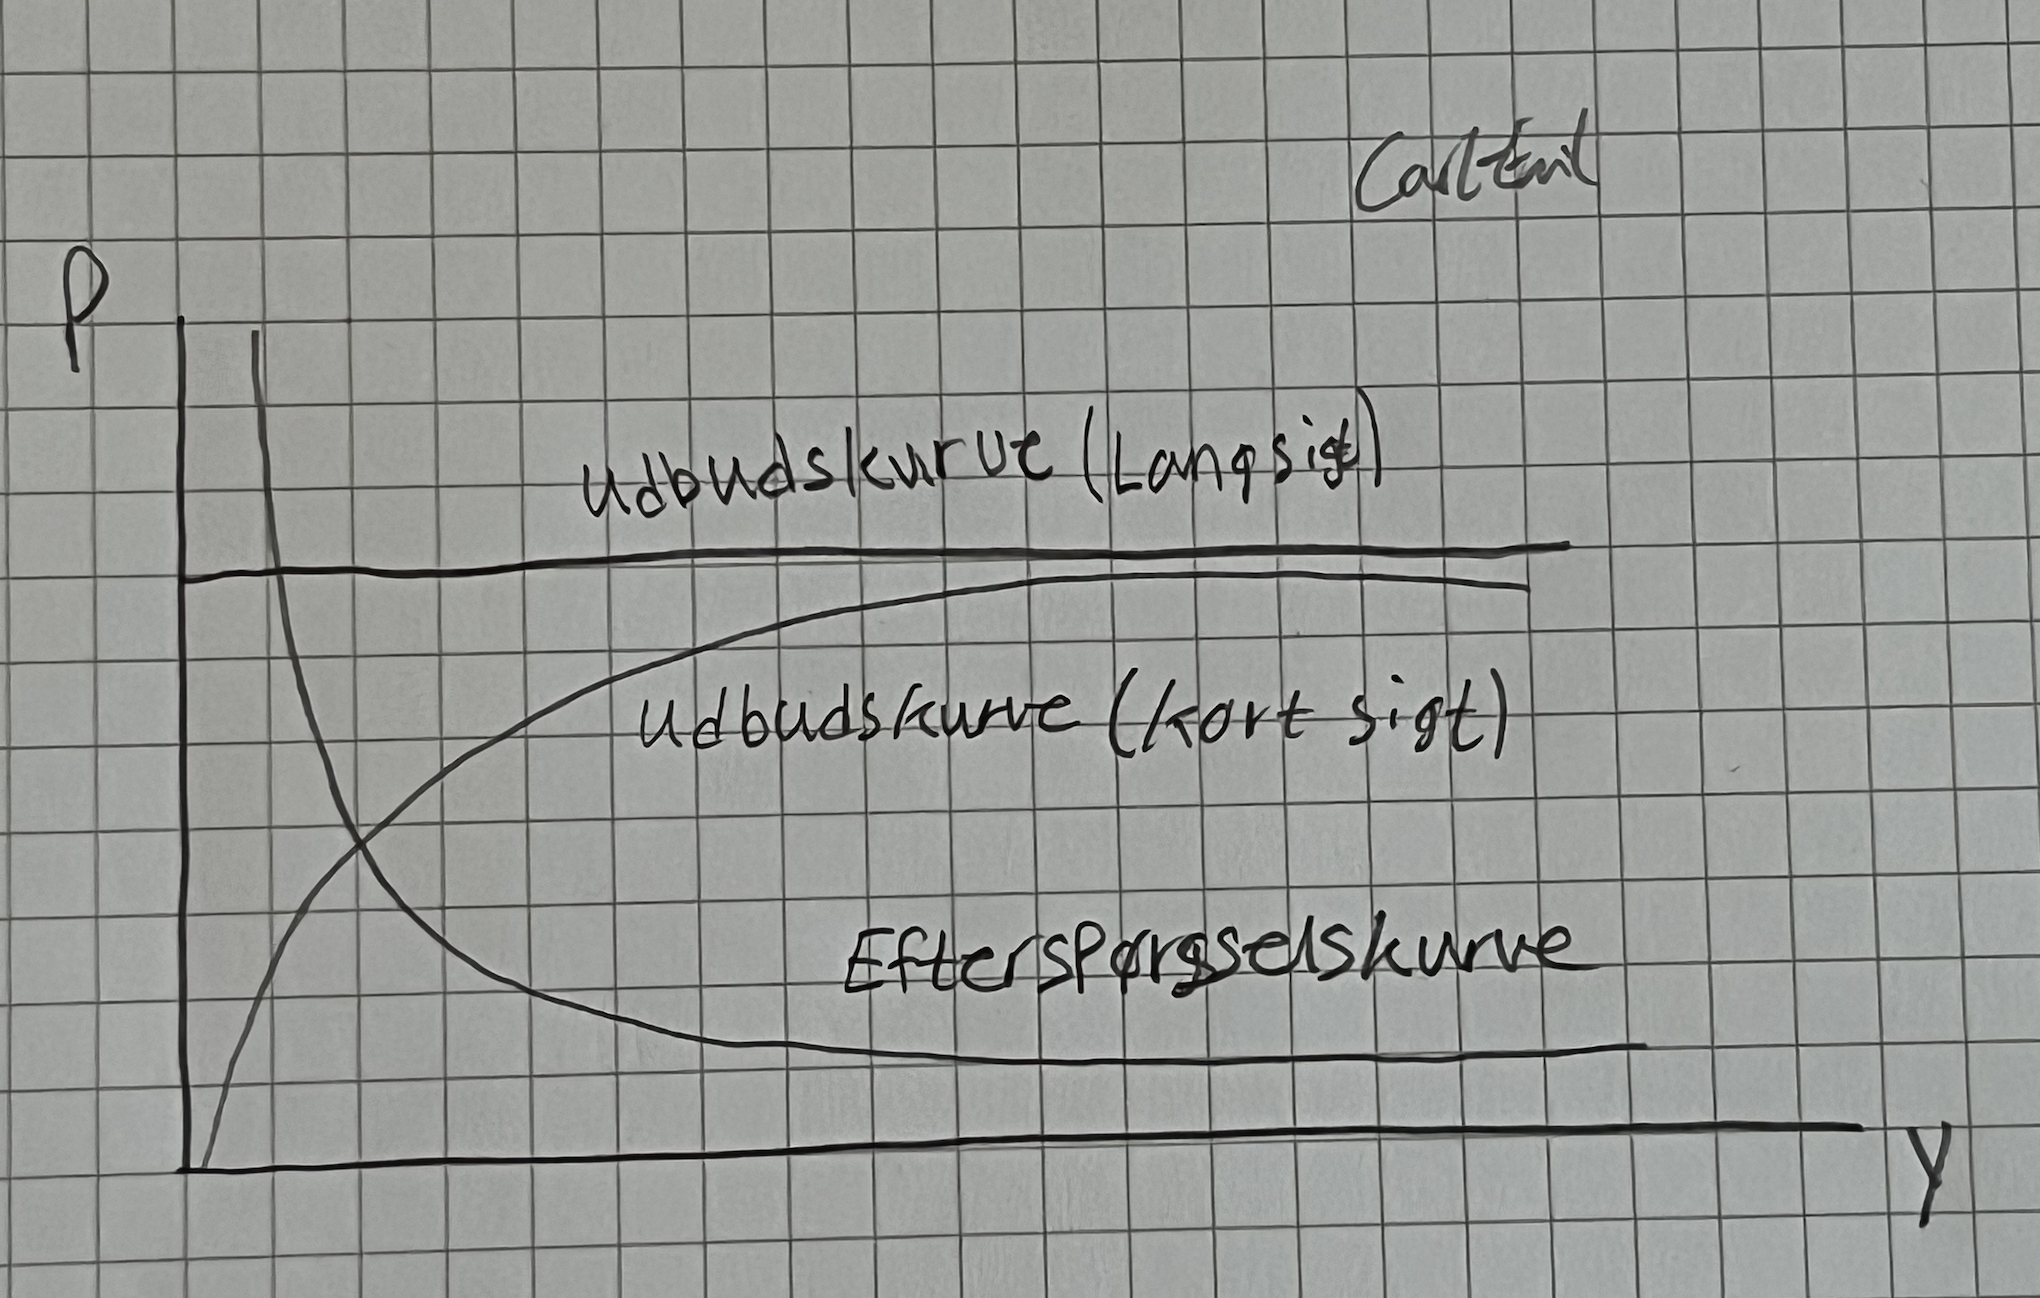
\includegraphics[scale=0.40]{2.png}
\end{center}






\end{document}
